
\section{Architecture and implementation}\label{sec:architecture}

\subsection{YETI standalone application}
YETI is usually launched on the command-line. A typical call of YETI is:
{\small
\begin{verbatim}
java yeti.Yeti -Java -yetiPath=. 
          -time=10mn -randomPlus
          -testModules=String:StringBuilder 
\end{verbatim}
}

The options used on this command-line have the following meaning: \texttt{-Java} 
indicates that the tested program is in Java, \texttt{-yetiPath=.} indicate that 
classes in the current directory (and its subdirectories) will be preloaded, 
\texttt{-time=10mn} indicates that the testing session will last 10 minutes, 
\texttt{-randomPlus} indicates that the strategy random+ will be used, and 
\texttt{-testModules=String:...} indicates that 
both \texttt{String} and \texttt{StringBuilder} will be tested.

While testing, traces of faults found are output to the terminal. For example:

{\small
\begin{verbatim}
Exception 5
java.lang.NullPointerException
 at java.lang.String.replace(String.java:2207)
\end{verbatim}
}

At the end of the testing sessions, YETI outputs generated test cases reproducing 
the faults found during the testing session as well.

Note that it is possible to avoid the overhead of keeping the 
traces in the system (and calculating the minimal test cases) by specifying 
\texttt{-nologs} to throw away all logs except exception traces, or 
\texttt{-rawlogs} to output the logs to the terminal. This comes at the cost of
not being able to generate test cases reproducing the failures, but only the 
exception traces. In an exploratory phase of the testing, this is generally the
way to use YETI.



\subsection{Architecture of the cloud implementation}
\begin{figure*}[h]
\begin{center}
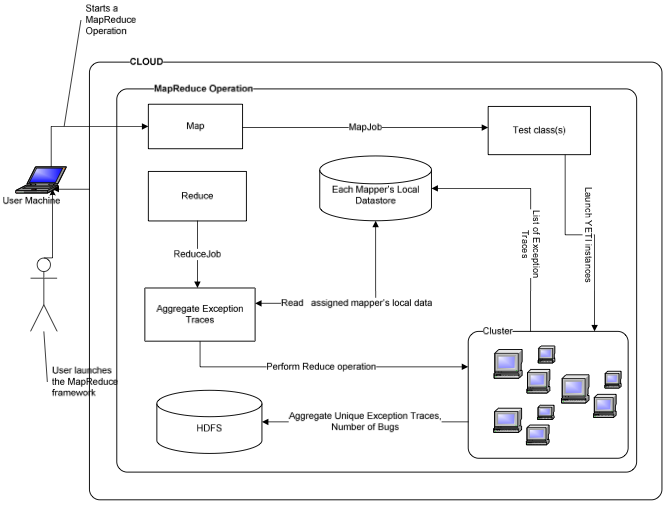
\includegraphics[width=14cm]{images/YetiCloud.png}
\end{center}
\caption{YETI cloud architecture.}\label{fig:architecture}
\end{figure*}


As figure~\ref{fig:architecture} shows, the main architecture of YETI ont he clouds 
relies on Hadoop, Apache's implementation of map/reduce. 

The main idea is that we use a very simple approach where testing jobs 
are described by simple command-line that would each launch YETI in standalone mode. 
Such jobs are then mapped to machines in the cloud. The order for the mapping 
is determined by the order used to write lines. 

The job is sent to the master as a jar file and then individual testing machines 
receive individual jobs to perform.

At the end of the testing session, all exception traces are sent back to the 
user machine through the reduce step by storing them into the Hadoop Distributed File 
System. Each of the traces is then stored separately and available to the software 
tester.


\subsection{Evaluation}

We only ran preliminary evaluations.

We evaluated our approach using the Amazon EC2 cloud\footnote{}.
We performed 20-minute jobs in less than 5 minutes, with outputting 
comparable results with executing standalone versions.

By using the cloud we can drastically improve the performances of YETI.
While we did not run experiments with more open security models, 
YETI jobs were run on one-shot Ubuntu virtual machines. This also solves
the potential security issues for random testing.
